\chapter{Completed Formative Work: Connectome Visualization}
\label{ch:connectome}

The second design study of this proposed dissertation is a two year collaboration with neuroscientists who were trying to reverse engineer the retina at a cellular level. They were part of an academic laboratory at the Moran Eye Center, University of Utah. They worked on descriptive science but their long term goals were to understand neurodegenerative diseases and to create therapies for those diseases~\cite{Anderson2010}. We used a creativity workshop early in the project to learn how visualization could help their analysis. Based on this workshop's results, we focused on analyzing connectivity in large multivariate graphs --- our collaborators needed to analyze connectivity in a {\bf connectome}, a graph of neurons (nodes) connected by synapses (edges). To support their analysis, we created two new visualization techniques and realized those techniques in a prototype visualization tool.

This design study is a formative project of this proposed dissertation as it provides important practical experience using a creativity workshop. From this experience we started meeting with other visualization researchers to identify best practices for future creativity workshops. The anticipated creativity workshop framework resulted from those conversations. 

In the remainder of this chapter, we discuss this project's contributions, summarize the novel visualization techniques, reflect on the creativity workshop, and list the resulting publications.

\section{Contributions}

This project had five contributions: 1) a set of five requirements for visualization software to support connectivity analysis; 2) two new visualization techniques that summarize graph connectivity --- the connectivity matrix and the intermediate node table; 3) a prototype open source implementation of those techniques called Graffinity; 4) a reflection on the use of creativity workshops that inspired this proposed dissertation; and 5) the validation of our tools as they were used to discover new circuitry between cells in the retina~\cite{Lauritzen2016}.

In the next section, we briefly describe contributions \#2 and \#3. Please see the publications at this chapter's end for more details about all of the contributions.

\section{Graffinity: Visualizing Connectivity in Large Graphs}

We focused on supporting connectivity analysis, reasoning about the direct and indirect connections between nodes, based on paths, and potentially considering node and edge attributes~\cite{Lee2006}. For example, consider a large graph of airports (nodes) connected by flights (edges). An analyst may be interested in how the airports of two regions are connected, allowing for one or more layovers and accounting for attributes such as flight delay. Similarly, our collaborators wanted to understand how different sets of cells were connected by paths accounting for attributes such as cell type or synapse weight. 

Standard graph visualization techniques are not effective for connectivity analysis in large graphs. Node-link diagrams are helpful in judging connectivity but they degenerate to hairballs beyond about 50 nodes~\cite{Shneiderman2005}. Adjacency matrices also do not scale to large graphs and are only suitable to judge direct connections between nodes as they require tedious manual indirection between rows and columns to follow paths~\cite{Ghoniem2005}. 

A key approach to realize scalable graph visualization are queries: instead of displaying the whole graph, only a relevant subset is shown. Query-based techniques for analyzing connectivity in graphs, however, can also easily suffer from cluttering if the query result is big enough.

We proposed two new query-based visualization techniques that provide a scalable overview of graph connectivity without the need for manual tracing or indirection: the connectivity matrix and the intermediate node table. The connectivity matrix is an adjacency matrix generalized to show path connectivity. It summarizes paths based on their starting and ending nodes. The intermediate node table reveals information about the middle nodes that is hidden by the connectivity matrix. These two techniques provide a scalable overview of connectivity as seen in the prototype implementation of Graffinity, shown in Figure~\ref{fig:04_graffinity}. Please see our paper~\cite{Kerzner2017} for a full description of these techniques, example usage with a flight dataset, and validating case studies in connectomics analysis. 

\section{Creativity Workshop Reflection}

We started this collaboration with unstructured interviews and contextual inquiry~\cite{Holtzblatt1993} to understand our collaborator's analysis needs, but we found three limitations with these methods. First, we identified seemingly disparate needs as each analyst was interested in specific research questions. This is a common intellectual challenge when working in large organizations with specialized analysts~\cite{Sedlmair2010}. Second, we were not able to meet with senior analysts --- e.g., professors --- because they delegated our meetings to junior analysts --- e.g., post docs and graduate students. Third, we faced interpersonal challenges as some analysts were not necessarily engaged in our collaboration. We struggled to understand our collaborator's analysis needs due to these challenges.

We decided to use a creativity workshop to identify the shared needs of our collaborators. At first, we considered an unstructured meeting with analysts, but we did not know enough about the domain to plan one effectively. Instead, we ran a creativity workshop with eight of our collaborators, following the structure described by Goodwin et al.~\cite{Goodwin2013}. Its methods followed a diverge-converge pattern to explore a broad range of ideas and then to winnow the ideas and focus on the more interesting ones.

The workshop exposed shared analysis needs of our collaborators. In feedback on the workshop, the director of our collaborator's organization said \emph{``the structured meeting created consensus by exposing shared user needs."} We discovered that many analysts needed software to support reasoning about connectivity. The workshop also helped establish rapport and trust with our collaborators, as the director said the workshop's \emph{``interpersonal leveling and intense re-visiting of concepts made more team progress in a day than we make in a year of lab meetings."} Similarly, we estimated that the one day workshop produced data equivalent to six months worth of interviews and contextual inquiry.

\section{Conclusion and Publications}

In this design study, we proposed a set of requirements for connectivity analysis in large multivariate graphs. We created two new techniques to fulfill those requirements and implemented those techniques in a prototype tool called Graffinity. We validated Graffinity with case studies analyzing connectomics data.

This design study is a formative project of this proposed dissertation for two reasons. First, in our reflection on the workshop, we started working with six visualization researchers to find best practices for using creativity workshops in visualization design. Second, our use of a creativity workshop provides qualitative data for our proposed framework. 

This chapter will be formed from the following publications in the final dissertation:

\begin{itemize}
    \item technique paper in Computer Graphics Forum, presented at EuroVis 2017 ~\cite{Kerzner2017}
    \item results paper in the Journal of Comparative Neurology~\cite{Lauritzen2016}
\end{itemize}

\begin{figure}
 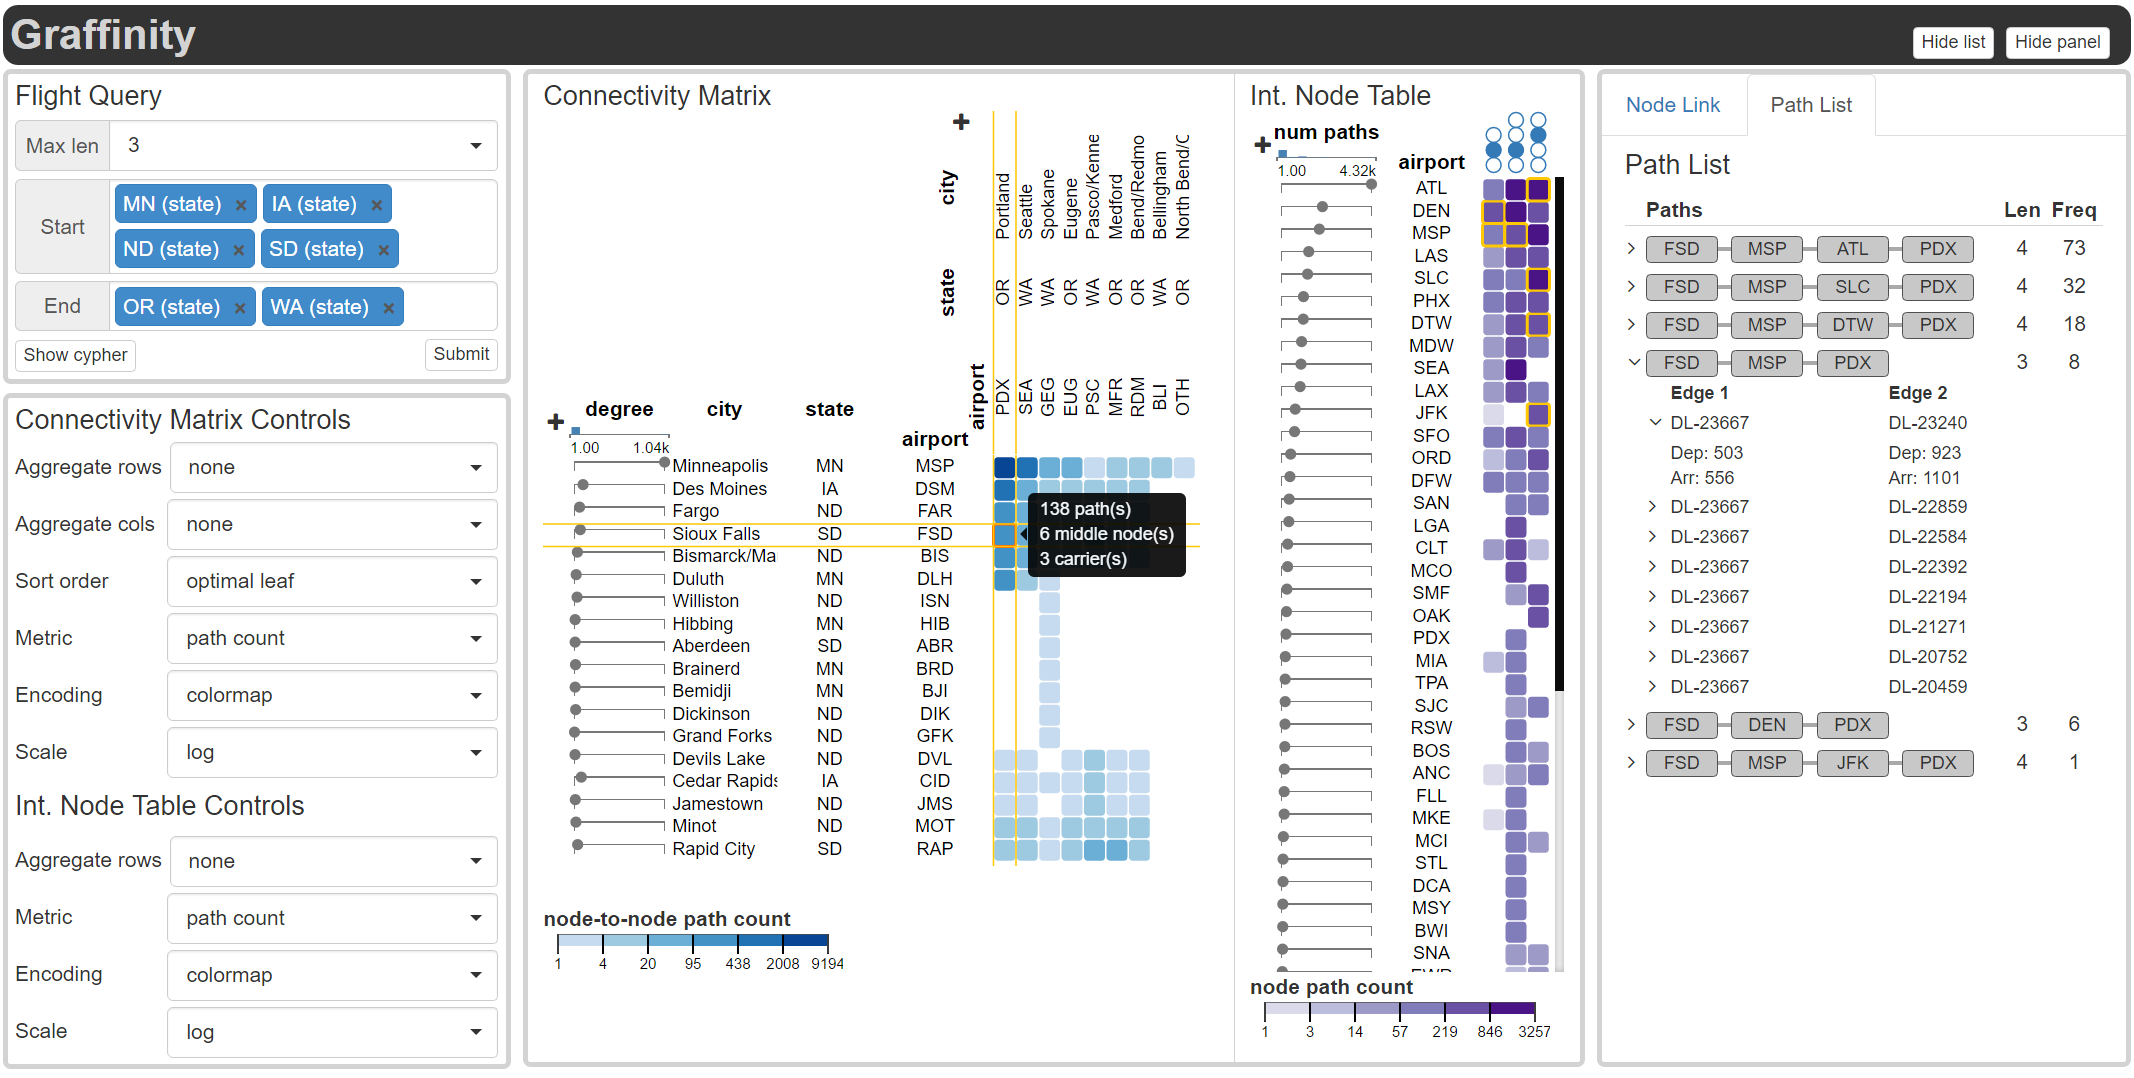
\includegraphics[width=\linewidth]{sources/figures/04_graffinity}
  \caption{Graffinity visualizing 11727 flight paths with length $\leq 3$ connecting states in the mid-western USA (Minnesota, Iowa, North Dakota and South Dakota) to states in the Pacific Northwest (Oregon and Washington). Graffinity consists of five views: the query interface, the connectivity matrix, the intermediate node table, and two views showing details about selected paths: the path list and the node-link view.  The 138 paths connecting the airport FSD (Sioux Falls, SD) to PDX (Portland, OR) are selected and displayed in the path list view.}
\label{fig:04_graffinity}
\end{figure}


